% ACL-ready figure for Smokemirror Pipeline
% Copy this into your paper's figure environment

\usepackage{tikz}
\usetikzlibrary{shapes.geometric, arrows.meta, positioning, fit, backgrounds, calc}

% Figure 1: Main Pipeline Overview (Full Width)
\begin{figure*}[t]
\centering
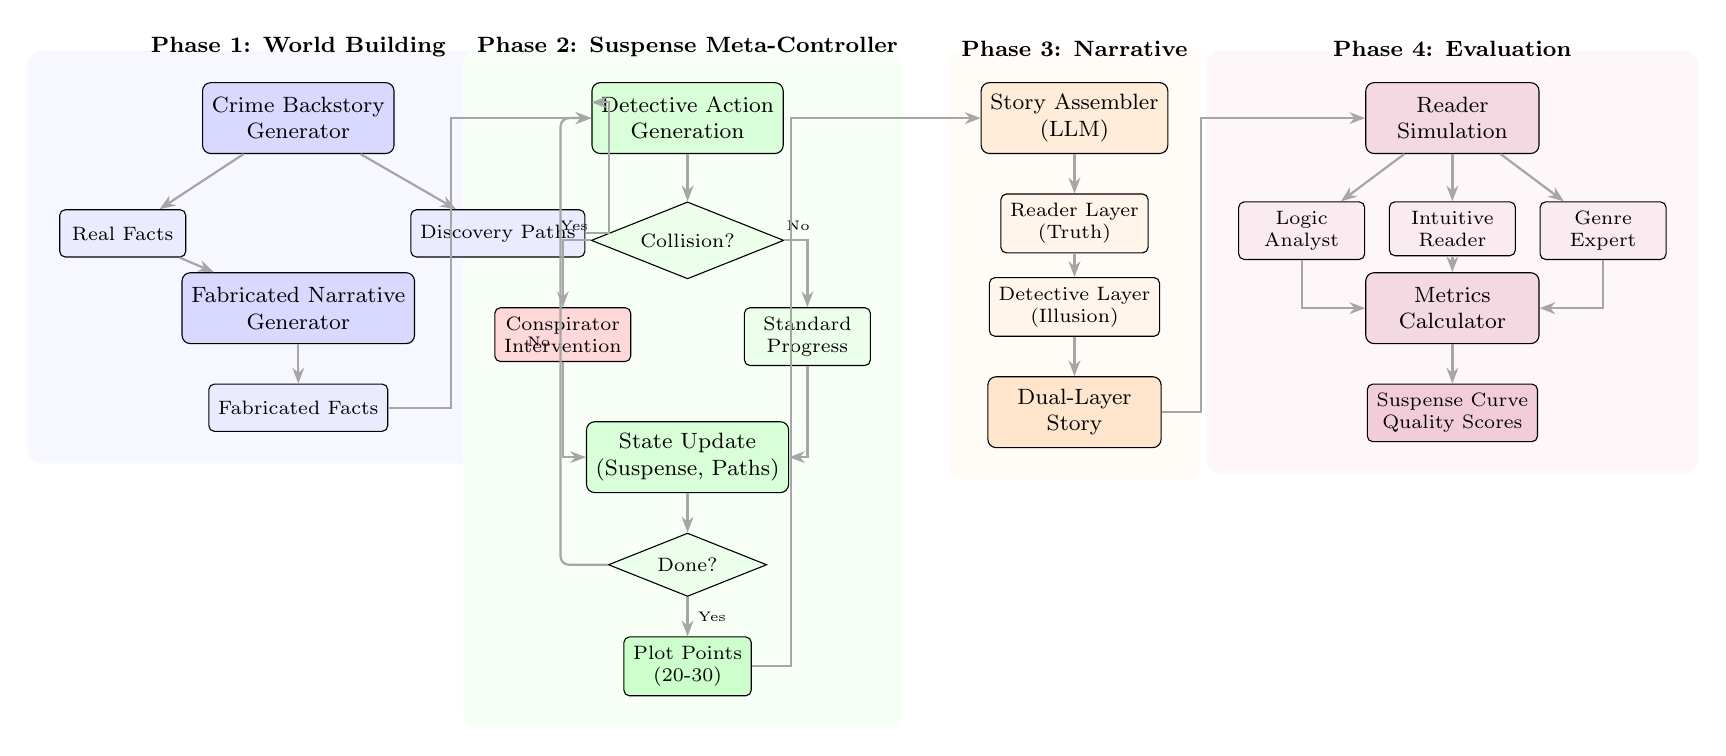
\begin{tikzpicture}[
    node distance=0.5cm and 0.8cm,
    mainbox/.style={rectangle, draw, rounded corners=3pt, minimum width=2.2cm, minimum height=0.9cm, align=center, font=\footnotesize},
    smallbox/.style={rectangle, draw, rounded corners=2pt, minimum width=1.6cm, minimum height=0.6cm, align=center, font=\scriptsize},
    phaselabel/.style={font=\footnotesize\bfseries, text=black},
    decision/.style={diamond, draw, aspect=2.5, minimum width=1.2cm, font=\scriptsize},
    arrow/.style={-{Stealth[length=2mm, width=1.5mm]}, thick, draw=gray!70},
    looparrow/.style={-{Stealth[length=2mm, width=1.5mm]}, thick, draw=gray!70, rounded corners=3pt},
]

% ============ PHASE 1: World Building ============
\node[mainbox, fill=blue!15] (backstory) {Crime Backstory\\Generator};
\node[phaselabel, above=0.2cm of backstory] {Phase 1: World Building};

\node[smallbox, fill=blue!8, below left=0.7cm and 0.2cm of backstory] (realfacts) {Real Facts};
\node[smallbox, fill=blue!8, below right=0.7cm and 0.2cm of backstory] (paths) {Discovery Paths};

\node[mainbox, fill=blue!15, below=1.5cm of backstory] (fabgen) {Fabricated Narrative\\Generator};
\node[smallbox, fill=blue!8, below=0.5cm of fabgen] (fabfacts) {Fabricated Facts};

% Phase 1 arrows
\draw[arrow] (backstory) -- (realfacts);
\draw[arrow] (backstory) -- (paths);
\draw[arrow] (realfacts) -- (fabgen);
\draw[arrow] (fabgen) -- (fabfacts);

% ============ PHASE 2: Suspense Controller ============
\node[mainbox, fill=green!15, right=2.5cm of backstory] (detective) {Detective Action\\Generation};
\node[phaselabel, above=0.2cm of detective] {Phase 2: Suspense Meta-Controller};

\node[decision, fill=green!8, below=0.6cm of detective] (collision) {Collision?};

\node[smallbox, fill=red!15, below left=0.6cm and 0.1cm of collision] (intervention) {Conspirator\\Intervention};
\node[smallbox, fill=green!8, below right=0.6cm and 0.1cm of collision] (progress) {Standard\\Progress};

\node[mainbox, fill=green!15, below=1.8cm of collision] (state) {State Update\\(Suspense, Paths)};

\node[decision, fill=green!8, below=0.5cm of state] (continue) {Done?};

\node[smallbox, fill=green!20, below=0.5cm of continue] (plotpoints) {Plot Points\\(20-30)};

% Phase 2 arrows
\draw[arrow] (detective) -- (collision);
\draw[arrow] (collision) -| node[above, font=\tiny, pos=0.3] {Yes} (intervention);
\draw[arrow] (collision) -| node[above, font=\tiny, pos=0.3] {No} (progress);
\draw[arrow] (intervention) |- (state);
\draw[arrow] (progress) |- (state);
\draw[arrow] (state) -- (continue);
\draw[arrow] (continue) -- node[right, font=\tiny] {Yes} (plotpoints);

% Loop back arrow
\draw[looparrow] (continue.west) -- ++(-0.6,0) |- node[left, font=\tiny, pos=0.25] {No} (detective.west);

% Connect Phase 1 to Phase 2
\draw[arrow] (fabfacts.east) -- ++(0.8,0) |- (detective.west);
\draw[arrow] (paths.east) -- ++(0.3,0) |- ([yshift=0.2cm]detective.west);

% ============ PHASE 3: Story Assembly ============
\node[mainbox, fill=orange!15, right=2.5cm of detective] (assembler) {Story Assembler\\(LLM)};
\node[phaselabel, above=0.2cm of assembler] {Phase 3: Narrative};

\node[smallbox, fill=orange!8, below=0.5cm of assembler] (readerlayer) {Reader Layer\\(Truth)};
\node[smallbox, fill=orange!8, below=0.3cm of readerlayer] (detectivelayer) {Detective Layer\\(Illusion)};

\node[mainbox, fill=orange!20, below=0.5cm of detectivelayer] (story) {Dual-Layer\\Story};

% Phase 3 arrows
\draw[arrow] (assembler) -- (readerlayer);
\draw[arrow] (readerlayer) -- (detectivelayer);
\draw[arrow] (detectivelayer) -- (story);

% Connect Phase 2 to Phase 3
\draw[arrow] (plotpoints.east) -- ++(0.5,0) |- (assembler.west);

% ============ PHASE 4: Evaluation ============
\node[mainbox, fill=purple!15, right=2.5cm of assembler] (readsim) {Reader\\Simulation};
\node[phaselabel, above=0.2cm of readsim] {Phase 4: Evaluation};

\node[smallbox, fill=purple!8, below left=0.6cm and 0cm of readsim] (logic) {Logic\\Analyst};
\node[smallbox, fill=purple!8, below=0.6cm of readsim] (intuitive) {Intuitive\\Reader};
\node[smallbox, fill=purple!8, below right=0.6cm and 0cm of readsim] (genre) {Genre\\Expert};

\node[mainbox, fill=purple!15, below=1.5cm of readsim] (metrics) {Metrics\\Calculator};

\node[smallbox, fill=purple!20, below=0.5cm of metrics] (scores) {Suspense Curve\\Quality Scores};

% Phase 4 arrows
\draw[arrow] (readsim) -- (logic);
\draw[arrow] (readsim) -- (intuitive);
\draw[arrow] (readsim) -- (genre);
\draw[arrow] (logic) |- (metrics);
\draw[arrow] (intuitive) -- (metrics);
\draw[arrow] (genre) |- (metrics);
\draw[arrow] (metrics) -- (scores);

% Connect Phase 3 to Phase 4
\draw[arrow] (story.east) -- ++(0.5,0) |- (readsim.west);

% ============ Background Shading ============
\begin{scope}[on background layer]
    \node[fit=(backstory)(realfacts)(paths)(fabgen)(fabfacts),
          fill=blue!3, rounded corners=5pt, inner sep=0.4cm] {};
    \node[fit=(detective)(collision)(intervention)(progress)(state)(continue)(plotpoints),
          fill=green!3, rounded corners=5pt, inner sep=0.4cm] {};
    \node[fit=(assembler)(readerlayer)(detectivelayer)(story),
          fill=orange!3, rounded corners=5pt, inner sep=0.4cm] {};
    \node[fit=(readsim)(logic)(intuitive)(genre)(metrics)(scores),
          fill=purple!3, rounded corners=5pt, inner sep=0.4cm] {};
\end{scope}

\end{tikzpicture}
\caption{Overview of the \textsc{SmokeMirror} story generation pipeline. The system constructs dual-layer mystery narratives through four phases: (1) generating ground truth and fabricated facts, (2) iteratively creating plot points with collision detection for suspense management, (3) assembling prose with parallel reader/detective perspectives, and (4) multi-agent evaluation simulating different reader types.}
\label{fig:pipeline}
\end{figure*}


% ============================================================
% Figure 2: Collision Detection Detail (Single Column)
% ============================================================

\begin{figure}[t]
\centering
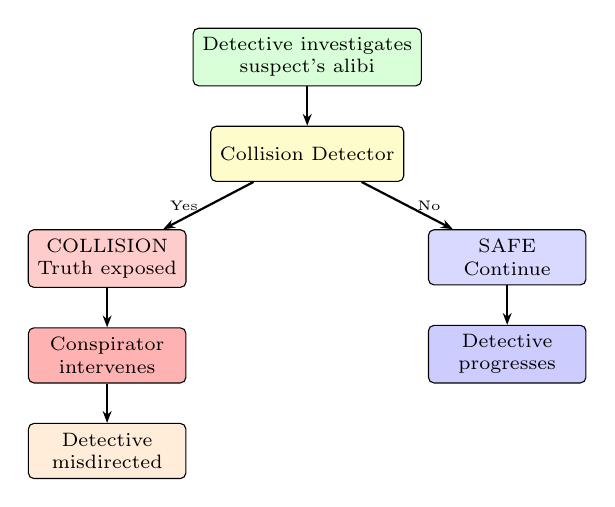
\begin{tikzpicture}[
    node distance=0.4cm,
    box/.style={rectangle, draw, rounded corners=2pt, minimum width=2cm, minimum height=0.7cm, align=center, font=\scriptsize},
    arrow/.style={-{Stealth[length=1.5mm]}, thick},
]

% Detective action
\node[box, fill=green!15] (action) {Detective investigates\\suspect's alibi};

% Collision check
\node[box, fill=yellow!20, below=0.5cm of action] (check) {Collision Detector};

% Two branches
\node[box, fill=red!20, below left=0.6cm and 0.3cm of check] (collision) {COLLISION\\Truth exposed};
\node[box, fill=blue!15, below right=0.6cm and 0.3cm of check] (safe) {SAFE\\Continue};

% Intervention
\node[box, fill=red!30, below=0.5cm of collision] (intervene) {Conspirator\\intervenes};

% Results
\node[box, fill=orange!15, below=0.5cm of intervene] (misdirect) {Detective\\misdirected};
\node[box, fill=blue!20, below=0.5cm of safe] (progress) {Detective\\progresses};

% Arrows
\draw[arrow] (action) -- (check);
\draw[arrow] (check) -- node[left, font=\tiny] {Yes} (collision);
\draw[arrow] (check) -- node[right, font=\tiny] {No} (safe);
\draw[arrow] (collision) -- (intervene);
\draw[arrow] (intervene) -- (misdirect);
\draw[arrow] (safe) -- (progress);

\end{tikzpicture}
\caption{Collision detection mechanism. When the detective's action threatens to expose the truth, a conspirator intervenes to maintain the cover-up.}
\label{fig:collision}
\end{figure}


% ============================================================
% Figure 3: Dual-Layer Narrative Structure (Single Column)
% ============================================================

\begin{figure}[t]
\centering
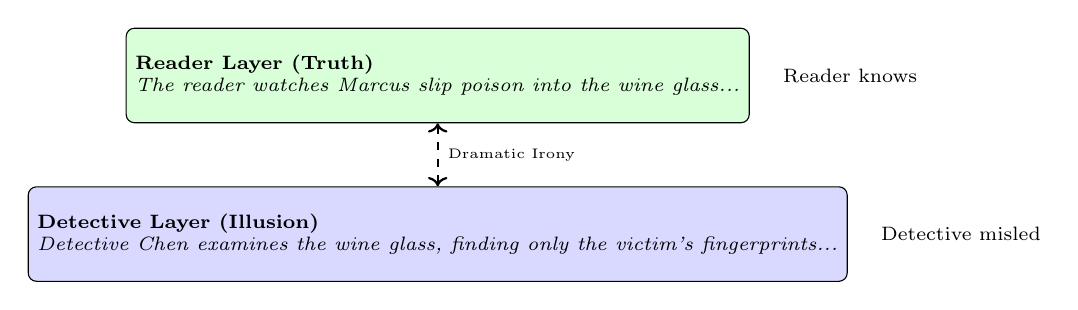
\begin{tikzpicture}[
    node distance=0.3cm,
    layer/.style={rectangle, draw, rounded corners=3pt, minimum width=6cm, minimum height=1.2cm, align=left, font=\scriptsize},
    arrow/.style={-{Stealth[length=1.5mm]}, thick, dashed},
]

% Reader layer (top)
\node[layer, fill=green!15] (reader) {
    \textbf{Reader Layer (Truth)}\\
    \textit{The reader watches Marcus slip poison into the wine glass...}
};

% Detective layer (bottom)
\node[layer, fill=blue!15, below=0.8cm of reader] (detective) {
    \textbf{Detective Layer (Illusion)}\\
    \textit{Detective Chen examines the wine glass, finding only the victim's fingerprints...}
};

% Connection
\node[font=\scriptsize, right=0.3cm of reader.east, anchor=west] (knows) {Reader knows};
\node[font=\scriptsize, right=0.3cm of detective.east, anchor=west] (misled) {Detective misled};

% Dramatic irony arrow
\draw[arrow, <->] (reader.south) -- node[right, font=\tiny] {Dramatic Irony} (detective.north);

\end{tikzpicture}
\caption{Dual-layer narrative structure. The reader observes both the truth and the detective's flawed investigation, creating sustained dramatic irony.}
\label{fig:dual-layer}
\end{figure}
